%!TEX root = main.tex

Over the past years, deep learning has contributed to dramatic advances in scalability and performance of machine learning~\cite{LeCun:2015}. One exciting application is the sequential decision-making setting of reinforcement learning (RL) and control. Notable examples include deep Q-learning \cite{Mnih:2015}, deep visuomotor policies \cite{levine2015end}, attention with recurrent networks \cite{Ba:2015}, and model predictive control with embeddings \cite{Watter:2015}. Other  recent successes include massively parallel frameworks~\cite{Nair:2015} and expert move prediction in the game of Go~\cite{Maddison:2015}, which produced policies matching those of Monte Carlo tree search programs, and squarely beaten a professional player when combined with search~\cite{alphago}.

In spite of this, most of the approaches for RL use standard neural networks, such as convolutional networks, MLPs, LSTMs and autoencoders. The focus in these recent advances has been on designing improved control and RL algorithms, or simply on incorporating existing neural network architectures into RL methods. Here, we take an \emph{alternative but complementary approach} of focusing primarily on innovating a neural network architecture that is better suited for model-free RL. This approach has the benefit that the new network can be easily combined with existing and future algorithms for RL. That is, this paper advances a new network (Figure~\ref{fig:duelnet}), but uses already published algorithms. 
%\begin{wrapfigure}{t!}{0.3\textwidth} 
%\vspace{-9pt}
\begin{figure}[b!]
\begin{center}
	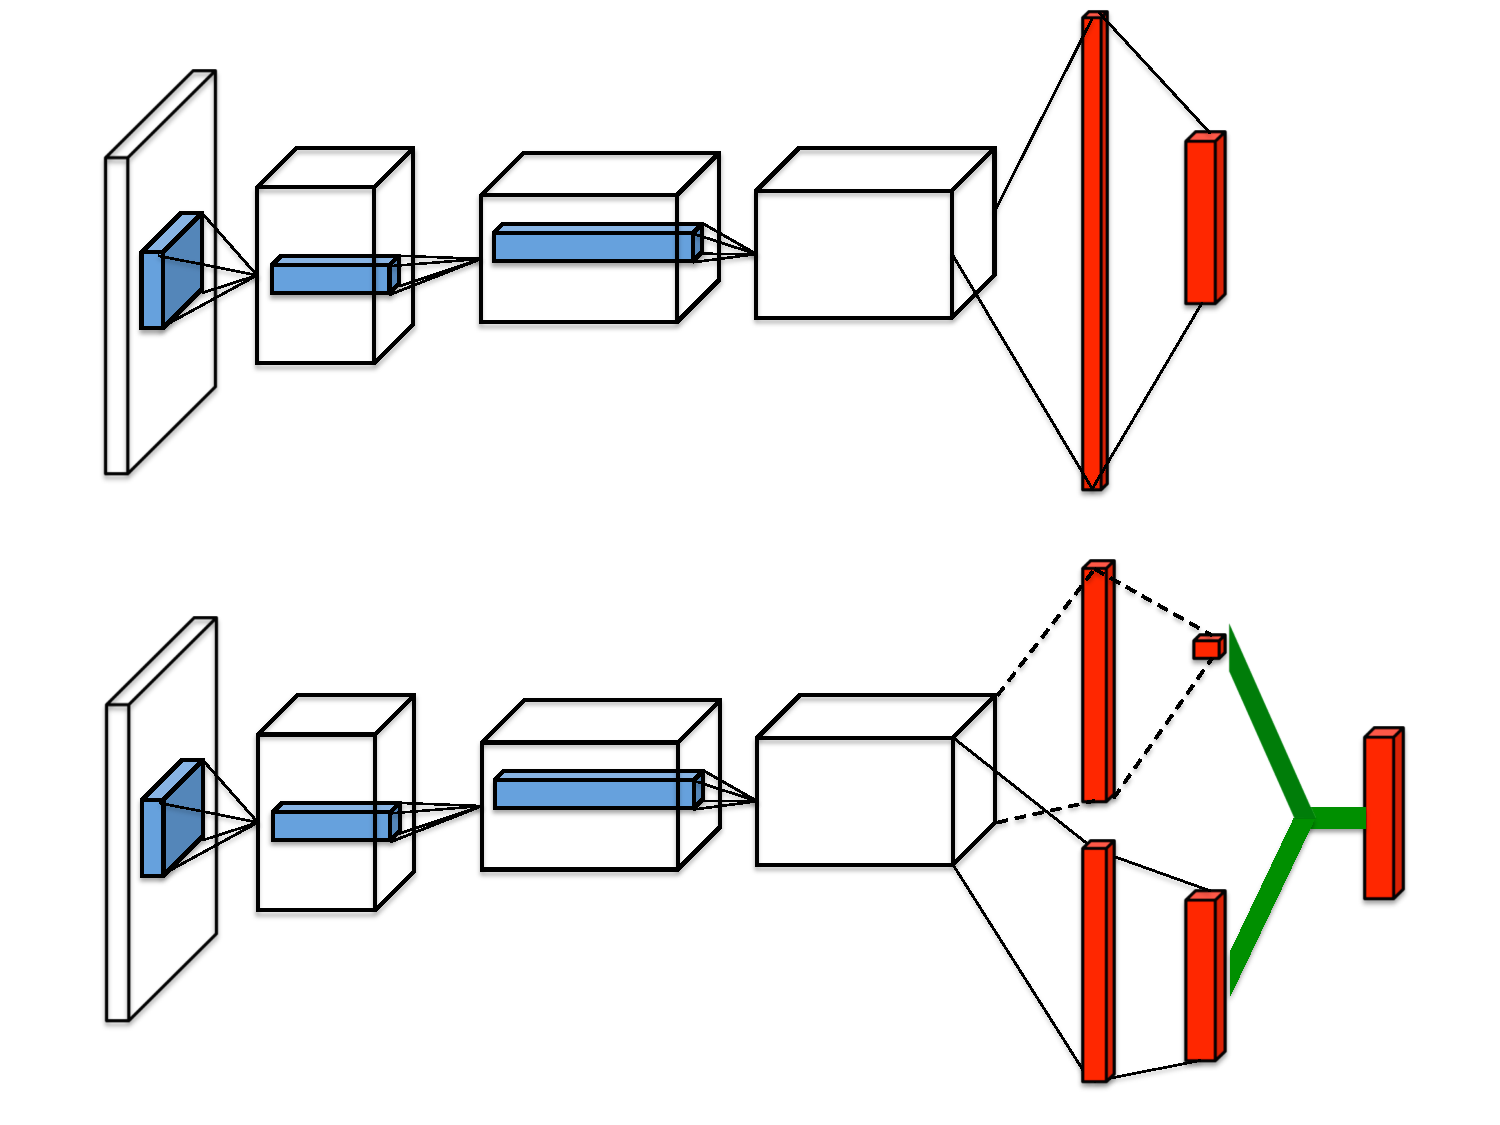
\includegraphics[scale=0.3]{./figs/duelingNet}
\end{center}
\vspace{-5mm}
\caption{A popular single stream $Q$-network ({\bf top}) and the dueling $Q$-network ({\bf bottom}). The dueling network has two streams to separately estimate (scalar) state-value and the advantages for each action; the green output module implements equation (\ref{eq:combo2}) to combine them. Both networks output $Q$-values for each action.}
\label{fig:duelnet}
\end{figure}
%\vspace{-20pt}
%\end{wrapfigure}

The proposed network architecture, which we name the {\it dueling architecture}, explicitly separates the representation of state values and (state-dependent) action advantages. The dueling architecture consists of two streams that represent the value and advantage functions, while sharing a common convolutional feature learning module. The two streams are combined via a special aggregating layer to produce an estimate of the state-action value function $Q$ as shown in Figure~\ref{fig:duelnet}. This dueling network should be understood as a single $Q$ network with two streams that replaces the popular single-stream $Q$ network in existing algorithms such as Deep Q-Networks \citep[DQN;][]{Mnih:2015}. The dueling network automatically produces separate estimates of the state value function and advantage function, without any extra supervision. 
%The new special aggregator that makes this possible is described in Section 3.



Intuitively, the dueling architecture can learn which states are (or are not) valuable, without having to learn the effect of each action for each state. This is particularly useful %when the agent encounters itself 
in states where its actions do not affect the environment in any relevant way. To illustrate this, consider the saliency maps shown in Figure~\ref{fig:saliency}\footnote{\url{https://www.youtube.com/playlist?list=PLVFXyCSfS2Pau0gBh0mwTxDmutywWyFBP}}.
These maps were generated by computing the Jacobians of the trained value and advantage streams with respect to the input video, following the method proposed by~\citet{Simonyan:2013}. (The experimental section describes this methodology in more detail.) The figure shows the value and advantage saliency maps for two different time steps. In one time step (leftmost pair of images), we see that the value network stream pays attention to the road and in particular to the horizon, where new cars appear. It also pays attention to the score. The advantage stream on the other hand does not pay much attention to the visual input because its action choice is practically irrelevant when there are no cars in front. However, in the second time step (rightmost pair of images) the advantage stream pays attention as there is a car immediately in front, making its choice of action very relevant. 
\begin{figure}[t!]
\begin{center}
{\sc \small \hspace{0.6cm} Value \hspace{1.8cm} Advantage } \\
	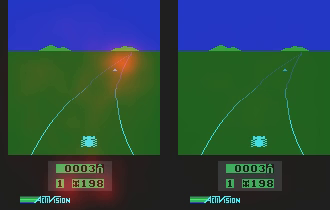
\includegraphics[scale=0.55]{./figs/enduro_color_1} \\
{\sc \small \hspace{0.6cm} Value \hspace{1.8cm} Advantage } \\
	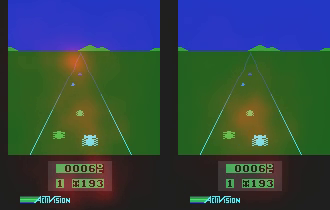
\includegraphics[scale=0.55]{./figs/enduro_color_2}
\end{center}
\caption{See, attend and drive: Value and advantage saliency maps (red-tinted overlay) on the Atari game Enduro, for a trained dueling architecture. The value stream learns to pay attention to the road. The advantage stream learns to pay attention only when there are cars immediately in front, so as to avoid collisions.}  
\label{fig:saliency}
\end{figure}

In the experiments, we demonstrate that the dueling architecture can more quickly identify the correct action during policy evaluation as redundant or similar actions are added to the learning problem. 

We also evaluate the gains brought in by the dueling architecture on the challenging Atari 2600 testbed. Here, an RL agent with the same structure and hyper-parameters must be able to play 57 different games by observing image pixels and game scores only. The results illustrate vast improvements over the single-stream baselines of~\citet{Mnih:2015} and~\citet{vanHasselt:2015}. The combination of
prioritized replay~\citep{Schaul:2015} with the proposed dueling network results in the new state-of-the-art for this popular domain.


%\begin{figure}[h!]
%\begin{center}
%	\includegraphics[scale=0.55]{./figs/nature_comp}
%\end{center}
%\caption{\label{fig:natureComp}Comparison against DQN \cite{mnih2015human}
%in human performance percentage. The gray dashed horizontal line marks human level 
%performance (75\% of expert score). The Dueling architecture beats DQN in 49 out of 57 games. 
%}
%\end{figure}

% By computing the Jacobians for the value and advantage branches of the dueling architecture, we obtain saliency videos illustrating which aspects of the input video stream the model thinks are valuable and which it thinks it must attend to when immediate action is needed. 
%  

%TODO(@Marc): MORE EXAMPLES OF RECENT DEEP LEARNING SUCCESSES + REFERENCES TO EXISTING ONES

% Adding a related work section in the short term for volume :)

\subsection{Related Work}

The notion of maintaining separate value and advantage functions goes back to \citet{Baird:1993}. In Baird's original advantage updating algorithm, the shared Bellman residual update equation is decomposed into two updates: one for a state value function, and one for its associated advantage function. Advantage updating was shown to converge faster than Q-learning in simple continuous time domains in~\cite{Harmon:1995}. Its successor, the advantage learning algorithm, represents only a single advantage function~\cite{Harmon:1996}.
%One of the goals of advantage learning is to increase the gap between the optimal action and suboptimal actions \cite{Baird:1999}.



% There is evidence that these Bellman residual algorithms can help stabilize when learning with gradient-based function approximation~\cite{Baird:1995,Baird:1999}. A very recent contribution is the consistent Bellman operator~\cite{Bellemare2015Persistent}, which also showed improvements in the Atari domain. We believe this improvement is independent and would be complementary, and we leave it as an interesting direction for future work.

%Actually, I don't know that citing this one makes much sense...
%Advantage functions have also been used when learning parsers for structured prediction using inverse reinforcement learning~\cite{Neu:2009}.

The dueling architecture represents both the value $V(s)$ and advantage $A(s,a)$ functions with a single deep model whose output combines the two to produce a state-action value $Q(s,a)$. Unlike in advantage updating, the representation and algorithm are decoupled by construction. Consequently, the dueling architecture can be used in combination with a myriad of model free RL algorithms. 
%Moreover, the representation of value and advantage is very rich, incorporating shared deep feature learning modules.

%Unlike advantage updating, it does not require two separate update rules. Similar to advantage learning, the dueling network computes a single state-action value. However, w
%We are unaware of any work that attempts to model these functions {with a shared deep representation}.
%, and whose updates are controlled by common gradient.  

% While learning is still model-free as in deep Q-learning~\cite{Mnih:2015}, the network's internal representation of $V^{\pi}(s)$ acts as a simple local model for each state's policy value, as experience replay does on the larger scale~\cite{vanSeijen:2015}. This local value learning can then simplify learning $Q^{\pi}(s,a)$ values across similar actions in state $s$ by focusing on the relative differences for each action $a$ from $s$.


There is a long history of advantage functions in policy gradients, starting with \cite{Sutton:2000}.
As a recent example of this line of work, ~\citet{schulman2015advantage} estimate advantage values online to reduce the variance of policy gradient algorithms. 


There have been several attempts at playing Atari with deep reinforcement learning, including \citet{Mnih:2015,Guo:2014,Stadie:2015,Nair:2015,vanHasselt:2015,Bellemare2015Persistent} and \citet{Schaul:2015}. The results of \citet{Schaul:2015} are the current published state-of-the-art.



%TODO(@Marc): ADD REF TO SCHULMAN'S ADVANTAGE ESTIMATION + PARSING/IRL PAPER

%modeling these values within the representation could lead to better generalization across similar actions and lessen the burden of engineering algorithmic improvements. Furthermore, this construction could allow more complex (e.g. contextual) interactions to be learned between state and action values.


